 \documentclass[a4paper,12pt]{report}

\usepackage[utf8]{inputenc}
\usepackage[T1]{fontenc}
\usepackage{array}
\usepackage{amsmath}
\usepackage[english]{babel}
\usepackage{graphicx}
\usepackage[a4paper]{geometry}
\usepackage[colorlinks=true,urlcolor=blue,linkcolor=blue]{hyperref}
\usepackage{url}
\usepackage[nottoc,numbib]{tocbibind}
\usepackage{color}
\usepackage{epstopdf}
\usepackage{xcolor}
\usepackage[backend=biber,style=phys]{biblatex}
\usepackage{lipsum}
\usepackage[capbesideposition={right,center}]{floatrow}

\addbibresource{../Bibliography.bib}
\makeatletter
	\renewcommand{\thechapter}{\Roman{chapter}}
\makeatother

\newcolumntype{M}[1]{>{\centering\arraybackslash}m{#1}}

\floatsetup[table]{style=plaintop}

\begin{document}

\chapter{Growth and first characterization of Cr-doped CdTe quantum dots\label{Growth}}

%	The growth took place at Tsukuba University, in the team of Pr. Shinji Kuroda. The samples were grown with Molecular Beam Epitaxy (MBE) and Atomic Layer Epitaxy (ALE, for the QD layer), via individual Cd, Te, Zn, Mg and Cr cells. MBE and ALE are two complementary techniques for the growth of semiconductor device.
	During this thesis, we studied two types of magnetic quantum dots: self assembled QDs and strain free QDs. The self assembled are formed by the partial relaxation of the strain of a CdTe layer on a ZnTe substrate (Stranski-Krastanov dots). Strain free dots are formed by thickness variation of a CdTe /CdMgTe thin quantum well. The growth of Cr doped samples were done in Pr. Shinji Kuroda laboratory, in the University of Tsukuba. The Mn-doped samples were grown at Grenoble, in the CEA-CNRS joined team NPSC, by Dr. Herv\'e Boukari.
	
	We will focus in this chapter on the growth done at Tsukuba by Molecular Beam Epitaxy (MBE). We begin by giving some general explanation on the MBE process and the different tools that are used in it. We then go to the growth of the self-assembled Cr-doped quantum dots, detailing the preparation of the substrate, the growth, and discussing the first characterization of the samples. In the last section, we present two other kinds of sample we grew: samples with the possibility of applying an electric field on them, and the strain free dots. For each of them, we detail the growth process and present basic characterization. 
	
	\section{The Molecular Beam Expitaxy}	
	
	The samples we used are grown using epitaxy. It consists on depositing atoms or molecules on the surface of the sample. Each elements are deposited on top of each other, and the lattice parameter of the substrate in the plane is kept as long as no defect appears in the material. To achieve such a growth, we used a process called Molecular Beam Epitaxy (MBE), in which flux of elements are evaporated toward the sample, where each atom or molecule is deposited and crystallize. This is done using cells of elements heated to control their evaporation or until they reach sublimation.

	{\huge Inclure historique ici}	
	
	 They are kept in Knudsen cells, which consist of a crucibles of high-melting-point material with a low contaminating power (typically Pyrolytic Boron Nitride) wrapped in Tungsten filament which will act as heater. Each are closed by a shutter controlled by a computer.
	
	When the desired cell temperature is reached, said shutter is opened to let the element travel to the substrate. The chamber containing the substrate is kept in Ultra High Vacuum (about $10^{-8}$ Pa), in order to avoid contamination of the sample and get a mean free path of the gas long compared to distance to the sample. This process is illustrated on Fig.~\ref{MBEScheme}. Reaching the surface, the atoms diffuse before stopping, either having dissipated their kinetic energy through interaction with the surface, or (more commonly) being kept by island of previously deposited atoms. In the ideal case, the growth occur layer by layer, slowly (about 1 monolayer/s), giving a good control of the thickness of the grown material.
		
%	 This technique consist of heating cells containing the pure elements which will formed the semiconductor in order to sublimate or evaporate them, such as presented on Fig \ref{MBEScheme}. Once the element is at the right temperature, the cell is opened and the gas can travel in the chamber with a ballistic trajectory. The mean free path of this gas is long compared to the size of the cells and the chamber, allowing the atoms to condensate on the substrate without interacting before. Once reaching the surface, the atoms diffuse on it before stopping, either having dissipated their kinetic through interaction with the surface, or (more commonly) being kept by island of previously deposited atoms. In the ideal case, the growth occur layer by layer, slowly (about 1 monolayer/s), giving a good control of the thickness of the grown material.	

	\begin{figure}[h!]
	\begin{center}
		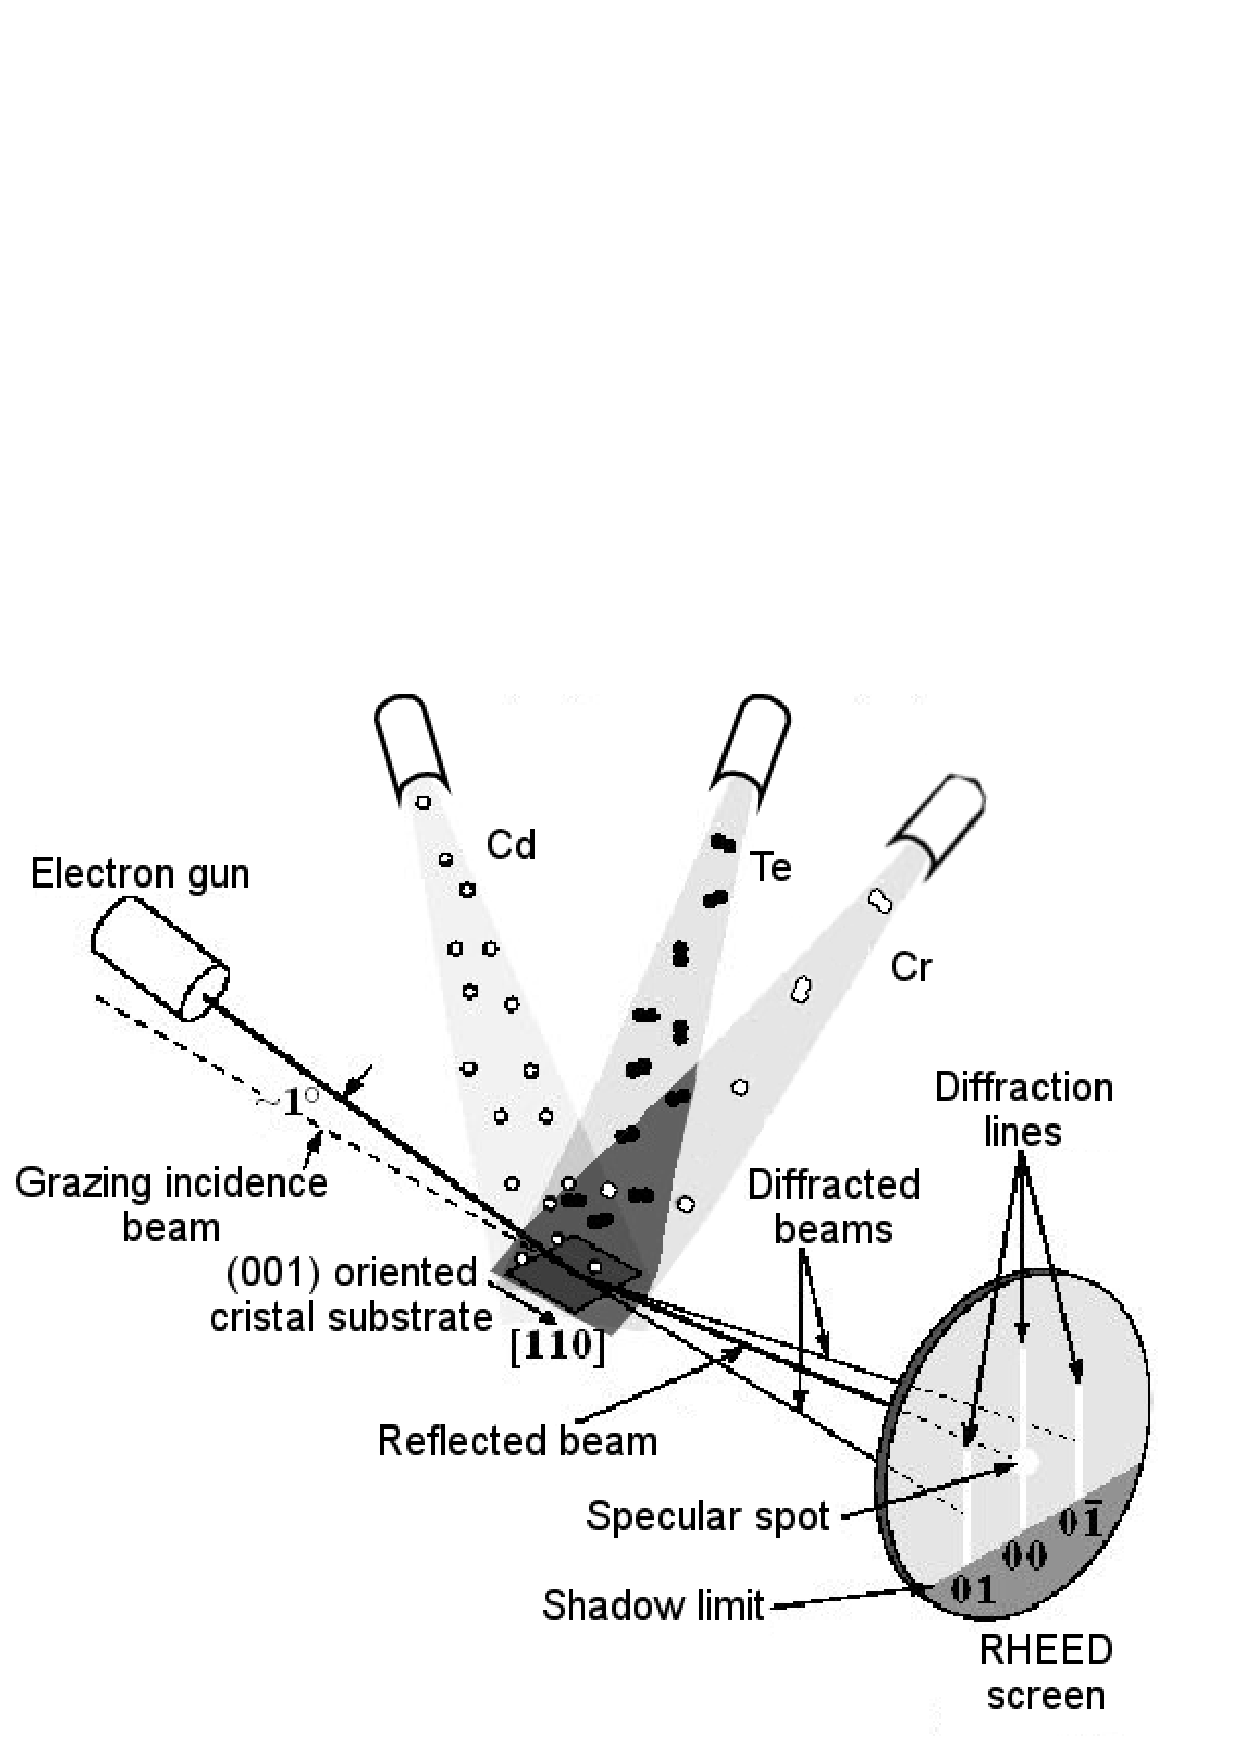
\includegraphics[width=10cm]{Pictures/MBE.png}
	\end{center}
	\caption{Scheme of a MBE chamber and the cells. An electron gun is also fixed to the chamber in order to probe the surface of the sample.}
	\label{MBEScheme}
	\end{figure}
	
%	Since MBE is a slow growth process, it ask for ultra-vacuum condition, in the order of $10^{-8}$ Pa, to avoid any contamination of the sample. Each raw material is contained in a Knudsen cell, which consist of a crucibles of high-melting-point material with a low contaminating power (typically Pyrolytic Boron Nitride) wrapped in tungsten filament which will act as heater. A small shutter close the container, and is controlled by computer along each recipe sequences.
	
	This necessity of Ultra High Vacuum kept the MBE to be developed before the end of the 1960s \cite{FirstMBE}, even though the idea was formalized at the end of the 19th century. This method offers a good control on the growth, which make it useful for the development of nanostructures. Depositing the materials layer by layer gives the possibility to grow really thin structure, and the transition between two materials can be made abrupt, over only a on or two monolayers (ML). Growing nano-structure is still the main use of MBE. However, this method is mainly used for research purpose, its slow growth speed and hard to fulfil growth conditions being an obstacle for the industrialization of the process.

%	Another mode of MBE is used during the growth of the samples: Atomic Layer Epitaxy (ALE) or Migration-Enhanced Epitaxy (MEE). In this mode, only one element is opened at a time, growing the sample really layer by layer. Between each opening, the sample is left under vacuum in order to relax the surface. A full cycle correspond to opening each cell once. For CdTe, a substrate temperature between 260$^{\circ}$C and 290$^{\circ}$C guaranty a growth of only 0.5 ML for each cycle~\cite{HMarALE}. This allow a small uncertainty on the substrate temperature while keeping a really good control on the growth of the sample.
%	\newline
	
%	In order to monitor each step of the growth, RHEED patterns of the sample surface were taken at different key moments. 
	The growth can be monitored with RHEED (Reflexion High-Energy Electron Diffraction). This technique requires a high vacuum, a given since MBE asks for ultra-high vacuum condition. An electron gun send a beam of high energy electron at a low angle, between 1$^{\circ}$ and 3$^{\circ}$, to the surface sample. This way, the electrons will only probe the surface of the sample, entering the material only on a 3 or 4 ML. Therefore the detected pattern directly gives information on the flatness and the crystallinity of the surface.
%	The detector, a CCD camera,  is set in order to collect only elastically scattered electrons.
	
	Incident electrons have a wave vector $\mathbf{k_i} = 2 \pi / \lambda_e$, with $\lambda_e$ the electron wavelength, typically 6 or 7 pm for an electron gun energy between 30 and 40 kV. Since only scattered diffraction is considered, the diffracted wave vector $\mathbf{k_f}$ as the same norm as the incident one $\mathbf{k_i}$. The Ewald's sphere has then a radius equal to the norm of $\mathbf{k_i}$. In the reciprocal space, the plane of diffraction are infinite line. So, in the case of a perfect crystal, with a perfect detector, the intersection with Ewald's sphere should be points. However, since the crystal may present some defect and neither the gun or the detector are perfect, the diffracted pattern shows lines.
	
	Once dots are grown, the surface become rough at the scale of the length of coherence of the beam. The electrons can interact with more layers while passing through the dots. This can be seen on the diffraction pattern, where lines become points.
	
%	These oscillations are also visible when growing a substrate in MBE mode. As each layer begin to grow, the intensity become dimmer, and then brighter as it is completed. Recording those oscillations, we can then calculate the growth speed from the number of oscillation occurring in a given time, converting this oscillation in ML, which thickness is known.
	
	%We are working with two sample holder, named "marked" and "unmarked", with slightly different temperature offset. The thermometer to measure the substrate temperature is placed at a few centimetre from the substrate holder, inducing another offset in the measured temperature.
	
	\section{Self-assembled CdTe/ZnTe quantum dots\label{SK}}
	
	\subsection{Substrate preparation}
	
		The samples were grown on ZnTe(100) substrates. In order to get the best surface to grow on, we need to clean the sample. Two cleaning methods were tested: etching of the substrate in a Bromide solution, and exposition of the substrate to a hydrogen radical plasma.

		The etching process was done in four steps. All of them, except the etching in Bromide-ethanol, occur in an ultrasonic cleaning device vibrating the sample at 43 kHz and last 3 minutes. We began with a cleaning in acetone, followed by one in ethanol. The third step was the actual etching: the substrate was put in a solution of Bromide-ethanol, with 3\% of Bromide, during 1 minute. We finally rinsed it in methanol. Once rinsed, we keep the sample in ethanol until fixing them to the sample holder. The growth usually occur the day after the cleaning, the sample being kept in the MBE load-lock chamber, under vacuum.
		
		Another type of cleaning of the surface was tried: using hydrogen radical (H$^*$) to remove the impurity at the surface. This was done to get a smoother surface directly in the chamber, to avoid any contamination that might occur during the transport from the etching room to the MBE chamber. The substrate was rinsed four times, first in acetone, then ethanol and then water, for a duration of 5 min with the cleaning device vibrating at 43 kHz, and finally 5 more minutes in water with the cleaning device vibrating at 23 kHz. It was then put in the MBE main chamber to be cleaned by H$^*$ radicals. In order to form the radical gas, a hydrogen gas was ionized in a chamber by a RF power source of 300 W and with a frequency of 13.6 MHz. This gas composition is optically checked by probing the emission of the Balmer series: for a pure hydrogen gas, peaks at 656 nm and 486 nm appear clearly. During the formation of this gas, the substrate temperature is raised to $400^{\circ}$C and we initiate its rotation. Once the plasma is formed, the valve to the main chamber is opened and the substrate is exposed to the plasma for 15 minutes. In order to check the quality of the surface, we look at the RHEED image, that should present stripes.
	
	\subsection{Stranski-Krastanov quantum dots growth\label{SKGrowth}}
	
	The targeted flux chosen for the growth of the CdTe/ZnTe QDs are presented in Tab.~\ref{FluxTempSK} for each cell used during the growth of strained QDs. These flux were measured via the pressure gauge inside the MBE chamber, and are therefore given in Beam Equivalent Pressure (BEP). It was shown that the best quality of ZnTe was achieved for a growth in excess of Zn~\cite{TeEffect}. Otherwise, vacancies appear in the bulk, optically visible, and the surface is more rough. Moreover, the adsorption power of the Zn is smaller than the Te. For these reason, we choose to grow the ZnTe barriers in excess of Zn.
	
	\begin{table}[h!]
	\begin{center}		
		\begin{tabular}{| c | c |}
			\hline
			Elements & Targeted BEP (Torr) \\ \hline
			Zn & $6.8\times10^{-7}$ \\
			Te & $4.5\times10^{-7}$ \\
			Cd & $4.5\times10^{-7}$ \\
			\hline
		\end{tabular}
		\caption{Targeted flux in Beam Equivalent Pressure (BEP) for each cell during the growth of the strained QDs.}
		\label{FluxTempSK}
	\end{center}
	\end{table}
	
	CdTe growth in MBE is \emph{auto-regulated}: if only one element is open, only a given quantity of material will be deposited and then the growth will stop until the other element is also deposited. The deposited quantity of material before the growth stop depends only on the substrate temperature. The flux of the elements has no influence on the quantity deposited at each cycle. The only consideration is whether enough material is deposited to reach the maximal thickness in a cycle. Therefore, the flux for both Te and Cd are chosen to be the same~\cite{HMarALE}.
	
	Beginning the growth, the substrate temperature was initially raised to $415^{\circ}$C. The Zn cell shutter was open starting at $360^{\circ}$C, in order to flatten the surface for the growth. While it took several minutes to raise the substrate temperature, only one Zn layer was deposited due to the auto-regulation of the growth. When the substrate temperature reach $415^{\circ}$C, the Te shutter was also open, in order to grow the ZnTe buffer layer. This thick ZnTe layer guaranteed us to the best possible surface for the growth of the QD layer~\cite{ChangZnTe}. The surface quality is checked by the RHEED picture, presenting clear lines (Fig.~\ref{RHEEDStep} (b)). Once done, we position the sample is order to have the specular spot on the RHEED screen, growing a few more ZnTe MLs to see the intensity variation of the reflected spot. The substrate temperature was then lowered to $295^{\circ}$C, the Zn cell being open until the temperature reach $360^{\circ}$C, preparing the growth of the dots doped with Cr atoms.
	
	\begin{figure}[h!]
	\begin{center}
		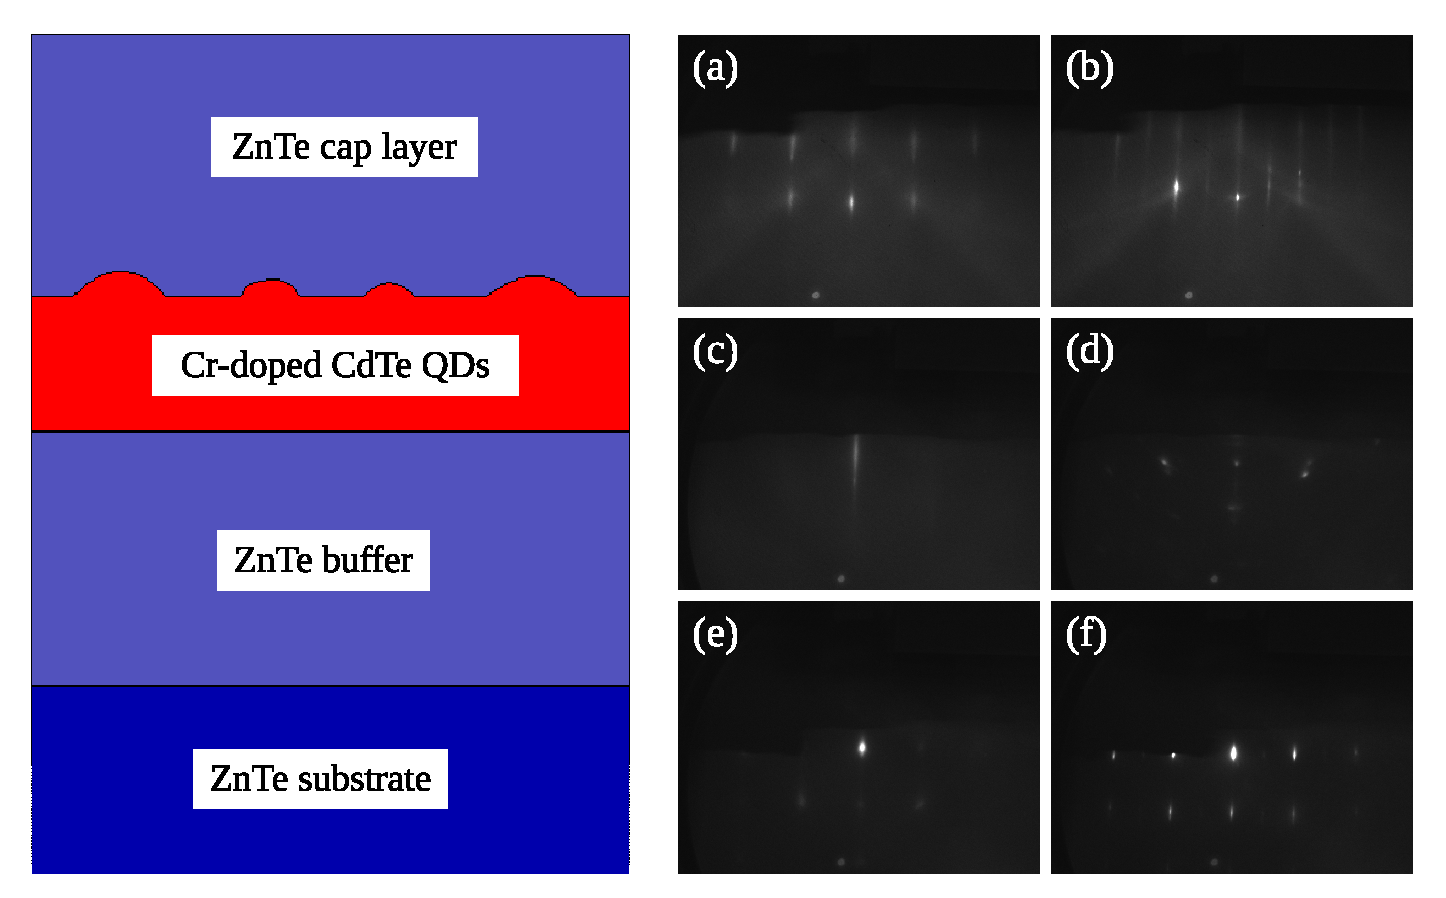
\includegraphics[width=14cm]{Pictures/RHEEDStep.eps}
	\end{center}
	\caption{Left: Layer structure of the strain Cr-doped CdTe QDs samples.
		Right: RHEED pattern taken at different key moment of the growth: (a) before the growth of the ZnTe buffer, (b) after the growth of the ZnTe buffer, (c) after the (Cd,Cr)Te ALE, (d) after the Te deposition, (e) during the Te evaporation (the picture was taken at T$_{substrate} = 177^{\circ}$C) and (f) after the growth of the ZnTe cap.}
	\label{RHEEDStep}
	\end{figure}
	
	Since the CdTe growth is auto-regulated, we can use a MBE mode called Atomic Layer Epitaxy (ALE) or Migration-Enhanced Epitaxy (MEE). In this mode, only one element is opened at a time, growing the sample layer by layer with good control on the growth. Between each opening, the sample is left under vacuum in order to relax the surface. This way, a really fine control of the growth and the deposited thickness is achieved. A full cycle correspond to opening each cell once. For CdTe, a substrate temperature between 260$^{\circ}$C and 290$^{\circ}$C guaranty a growth of only 0.5 ML for each cycle~\cite{HMarALE}. This allow a small uncertainty on the substrate temperature while keeping a really good control on the growth of the sample.
	
	The growth during ALE was monitored via the RHEED intensity. Focusing on the lowest angle reflected spot, called the specular spot, one can see small variations in the reflected intensity during the growth, such as presented on Fig.~\ref{RHEEDOsc}. This intensity is minimal when there is half a ML grown, and maximal when the ML is fully grown. This is due to the variation of reflectivity of the surface: maximal for a flat surface, minimal for a rough one. Therefore, a period of these oscillation is exactly the growth of a single monolayer~\cite{FirstRHEED,WoodRHEED}. We can also see the relaxation of a layer: the surface becomes then rougher, and the specular sport stays at low intensity.
	
	\begin{figure}[h!]
	\begin{center}
		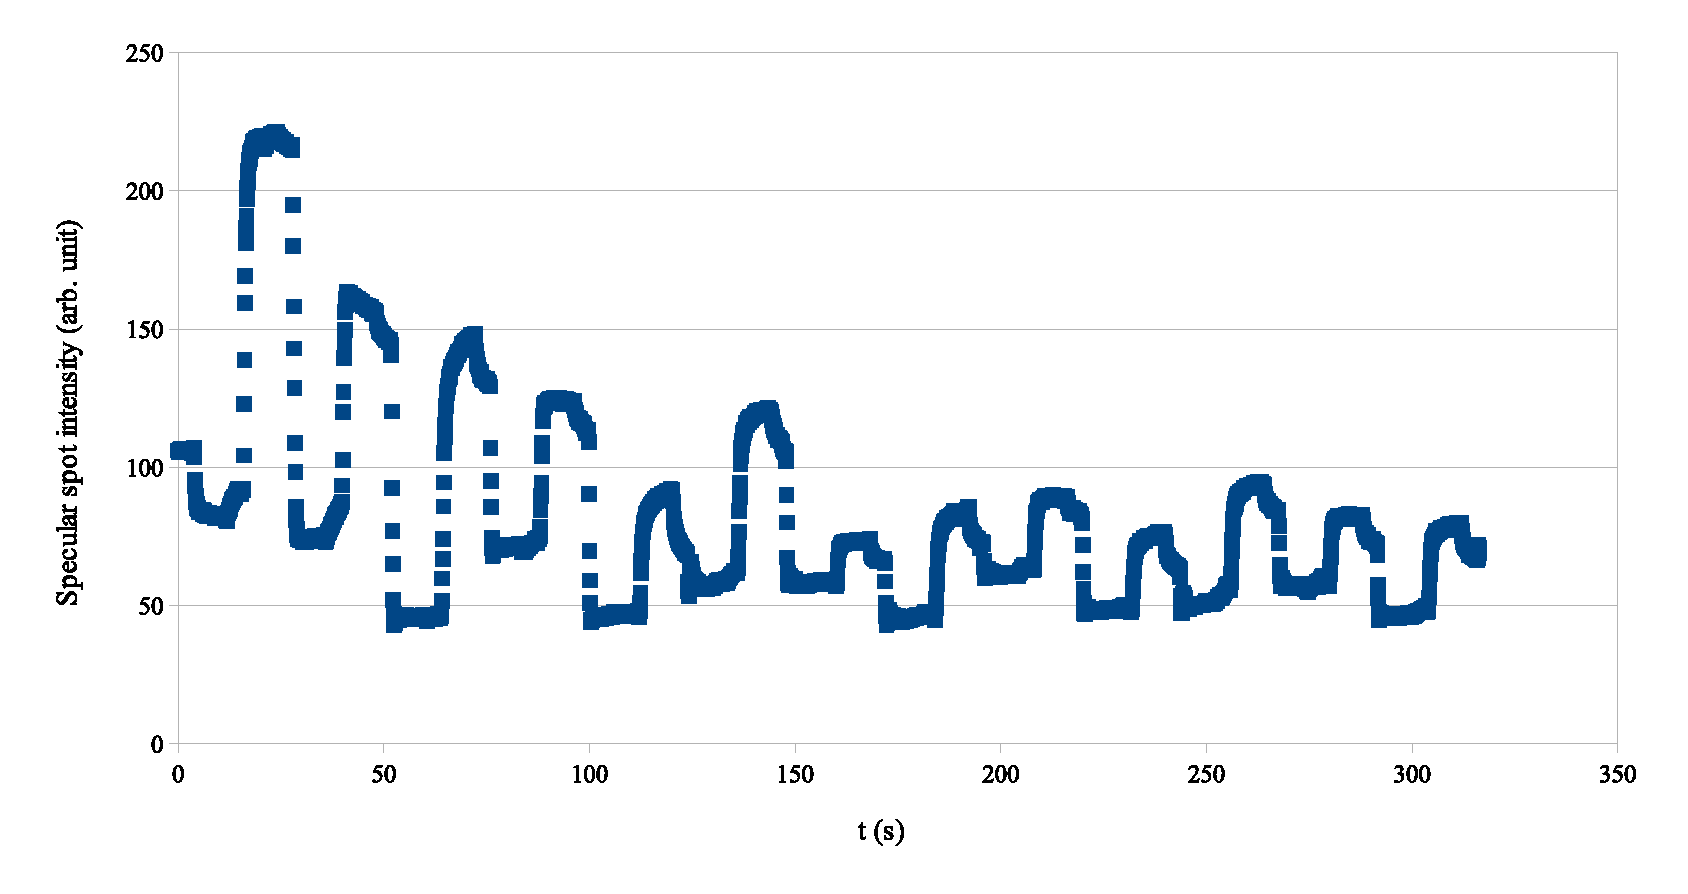
\includegraphics[width=14cm]{Pictures/SFDRheed.eps}
	\end{center}
	\caption{RHEED oscillation for the ALE of the strained dots.}
	\label{RHEEDOsc}
	\end{figure}
	
	One of the main goal of this work was to calibrate the Cr flux in order to embed only a single Cr atom in most of the QDs of the sample. A first guess is that the Cr density must be of the same order as the QDs density at the surface of the sample. This means a really small flux, with a BEP of the magnitude of $10^{-10}$ Torr, which is about one order lower than the main chamber pressure and therefore not measurable using the gauge pressure. The optimisation was done starting with the know how acquired in Grenoble on the Mn and trying to optimise it for the Tsukuba machine, through a feedback loop with the micro-PL characterization in Grenoble.

	This really small flux was achieved by heating the Cr cell around 1000$^{\circ}$C, low compared to its sublimation temperature, and opening the cell only once during the ALE, for only 5s. In order to have big enough QDs, emitting at right wavelengths, 6.5 ML of CdTe is the optimal thickness. However, the critical thickness of CdTe on ZnTe is 6.5 ML. Dislocations and defect will form in the layer for a higher thickness. Therefore, some samples were also grown with a 5.5 ML thickness in order to not get too close to the limit. At the chosen temperature, it correspond to either 13 cycles of ALE (for 6.5 ML) or 11 cycles (for 5.5 ML). The Cr cells was opened during the 7th cycle, halfway through the growth of the QD layer, in order to allow the Cr atoms to diffuse without going out the QD layers. The whole ALE recipe to grow the QDs layer is given in the Fig.~\ref{RecipeSK}.
	
	\begin{figure}[h!]
	\begin{center}
		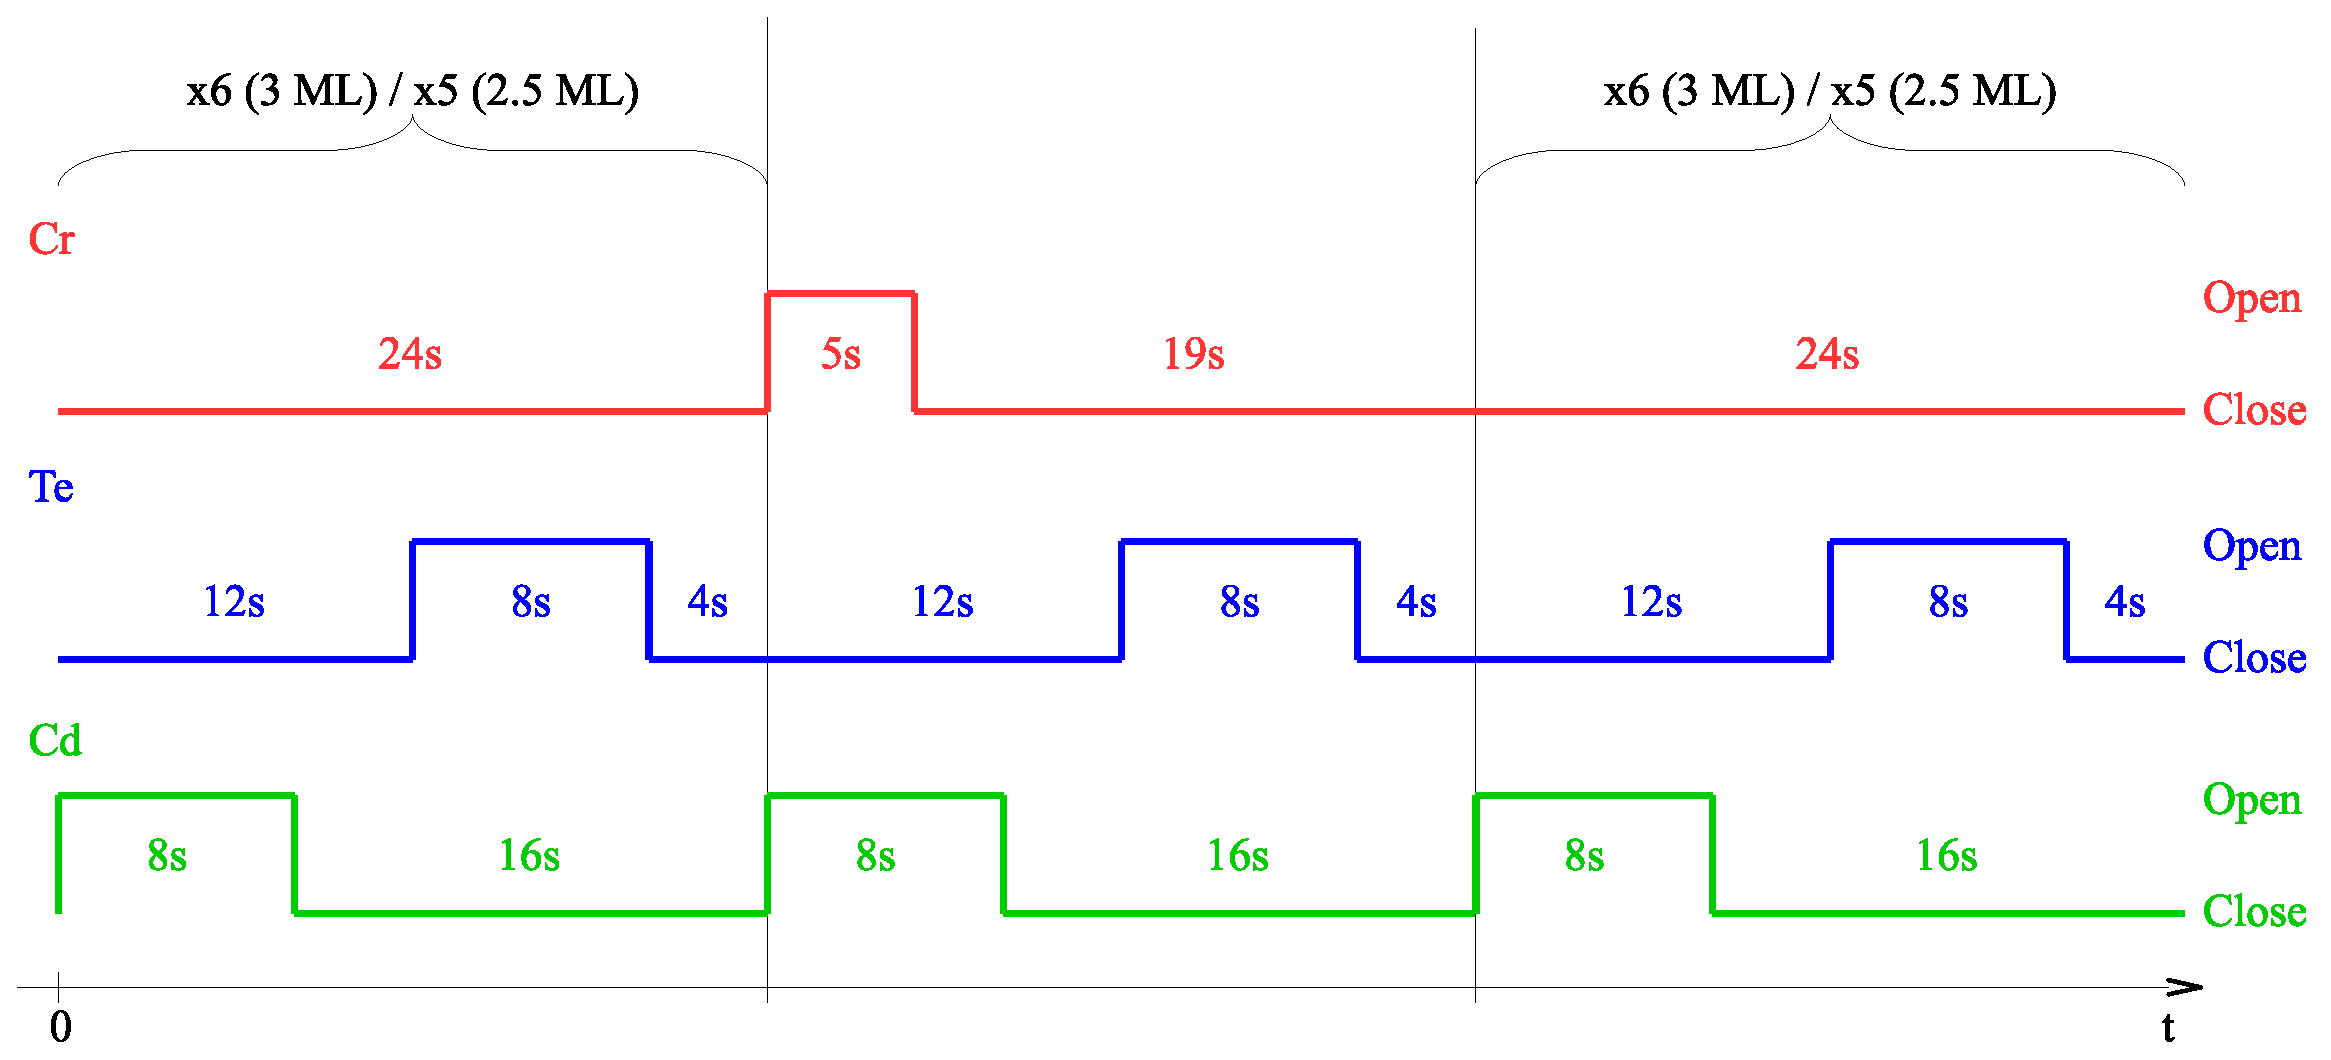
\includegraphics[width=14cm]{Pictures/RecipeSK.eps}
	\end{center}
	\caption{Opening and closing cycles of each cell for the ALE of strained (Cd,Cr)Te samples.}
	\label{RecipeSK}
	\end{figure}

	After the growth of the CdTe layer, we lowered the substrate temperature to $210^{\circ}$C to deposit an amorphous Te layer. It was deposited during 5 minutes. This step allows the CdTe layer to relax and form the quantum dots~\cite{TinjodMBE}. We then heated up the substrate again until $320^{\circ}$C, were we stayed for 20s in order to evaporate all the deposited Te~\cite{WojnarMBE}. If the dots were formed, we saw a spotty pattern like the one presented on Fig.~\ref{RHEEDStep} (f). The Zn and Te cells were then opened, while the substrate temperature was raised to $350^{\circ}$C in order to grow a protective layer above the QDs.
	
	\subsection{Optical characterization}
	
	The samples were studied in Grenoble, at the Neel Institute. A high refractive index hemi-spherical Solid Immersion Lens (SIL) was mounted on the sample before their study, to improve the spatial resolution and enhance the collection efficiency of a single dot photoluminescence (PL) in a low temperature (T = 5K) optical microscope.
	
	The characterization of the samples came in two times. First, we took macro-photoluminescence spectra, on a large energy range, typically between 1.8 and 2.3 eV, with a laser exciting at 2.9 eV. This allow us to test the luminescence of the sample: if the Cr concentration is too high, it may kill the PL of the dot layer, and thus it will not be seen in the macro-PL. If this luminescence is seen, the sample is then studied by micro-photoluminescence ($\mu$-PL), on a much narrower energy band (about 10 meV), in order to be able to study the dots individually. We scan randomly the sample, searching for dots. We judge the quality of the sample by the proportion of thin emission peaks versus broad ones, large quantity of broad peaks suggesting a high Cr concentration, and by the number of actual dots we found with single Cr embedded inside.
	
	\begin{table}[h!]
		\begin{center}
			\caption{List of samples where Cr-doped dots growth was successfully achieved.\label{SKsamples}}
			\begin{tabular}{M{2.5cm}|M{3cm}|M{2.7cm}|M{3.5cm}}
				Sample & Cleaning process & \# CdTe MLs & Targeted Cr concentration (\%) \\
				\hline
				dot334 & Br etching & 6.5 & 0.09 \\
				dot338 & Br etching & 6.5 & 0.05 \\				
				dot359 & Br etching & 6.5 & 0.11 \\
				dot363 & Br etching & 6.5 & 0.21
			\end{tabular}
		\end{center}
	\end{table}
	
	The samples where the Cr concentration was found to be correct are listed in Tab.~\ref{SKsamples}. The Cr concentration in the sample is only indicative and was estimated using the Cr flux. However, since the Cr flux was too low to be measured, we calculated it using Arrhenius law on flux measured at higher temperature. We see that correct samples were found for a large range of concentration. However, in dot338, we have a really probability to find Cr-doped dots. On the other hand, dot363, with the higher Cr targeted concentration, presents a lot of broad peaks. In all samples grown at higher Cr targeted concentration, the luminescence was too weak to study them properly. We can estimate that the good range of concentration is between 0.05\% and 0.20\%. Some more test have to be done in-between those concentration, especially around 0.10\%.
	
	\section{Other kind of samples}
		\subsection{Charge control samples\label{ChargedSample}}	
		
	The charge control samples are grown in order to be able to apply an electric field on the dot layer. The growth occurs on a p-doped ZnTe substrate. It gives the sample a conductive back. The growth was done in order to form Stranski-Krastanov dots, as described in the previous section. However, thinner buffer and cap layers were necessary in order to be able to apply a stronger electric field on the dot layer. We chose a thickness for the barrier between 150 nm and 200 nm.
	\begin{table}[h!]
		\renewcommand{\arraystretch}{1.5}
		\begin{center}
			\caption{Conductivity of the Au layer on GaAs for different deposition time.}
			\label{AuDep}
			\begin{tabular}{|M{4.5cm}|M{0.5cm} M{0.5cm} M{0.5cm} M{0.5cm} M{0.5cm} M{0.5cm}|}
				\hline
				Gold deposition time (s) & 15 & 20 & 25 & 30 & 35 & 60 \\ \hline
				Resistance ($\Omega$) & 300 & 80 & 25 & 20 & 0 & 0 \\ \hline
			\end{tabular}
		\end{center}
	\end{table}
	
	\begin{figure}[h!]
	\fcapside{\caption{Schema of the charge control structure, on a p-doped ZnTe substrate and with a thin, semi-transparent gold layer deposited on the surface. Electrode are glued on the surface and the back in order to apply a magnetic field. A SIL can be positioned on the surface in order to improve the spatial resolution and enhance the collection efficiency of a single dot photoluminescence (PL).}\label{ChargeContSample}}	
	{\begin{center}
		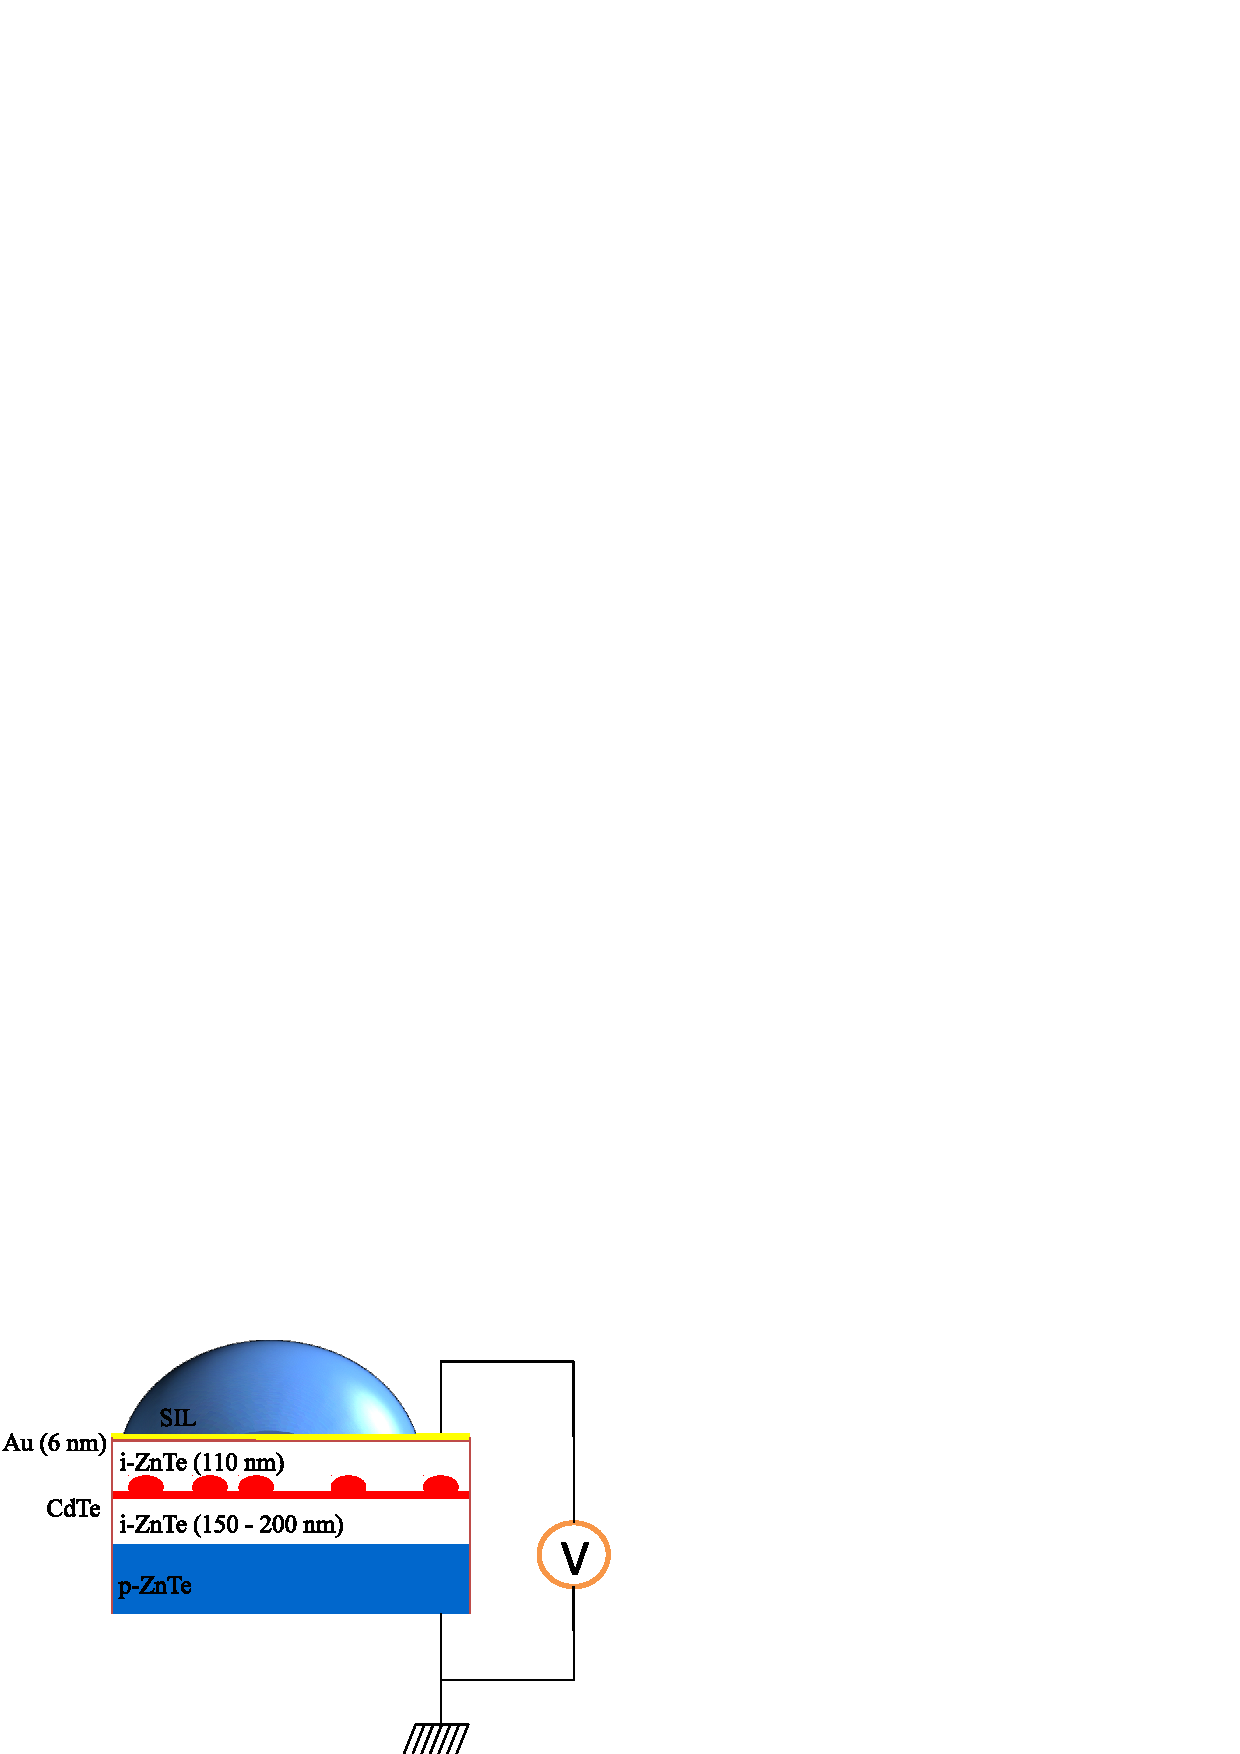
\includegraphics[width=7.3cm]{Pictures/ChargeContSample.png}
	\end{center}}
	\end{figure}
	
	The conductive surface was formed by a thin, semi-transparent gold layer, forming a Schottky junction with the sample cap layer. It was deposited by sputtering. The samples were kept in nitrogen atmosphere during the transport. The exposition time of the sample in the sputtering machine was calibrated using gold deposited on GaAs substrate. In order to keep a collection of the light emitted by the quantum, a thin layer was necessary. However, for the applied electric field to be uniform, we also needed a gold layer thick enough to be uniformly applied on the entire surface. Such a uniform layer means the resistance of the sample surface fall to 0 $\Omega$. Results of the resistance measurement are presented in Tab.~\ref{AuDep}. A deposition time of 35 s was chosen.
	
	Fig.~\ref{ChargeContSample} shows a schema of the sample as it was studied. Gluing electrode to these conductors, we are able to apply an electric field on the dot layer without inducing a current in at low voltage. A SIL was mounted to do the $\mu$-PL of single dot in order to improve the spatial resolution.
	
 	\subsubsection*{Optical characterization}
	
	We successfully grew these samples and studied them with $\mu$-PL. We were able to look at the luminescence of a dot and see the evolution of its PL under the application of a bias voltage. Fig.~\ref{ChargeVar} (a) presents the results of such an experiment.
%	 One can notice that all the emission energy of all the species change under application of an electric field.

	\begin{figure}[h!]
	\begin{center}
		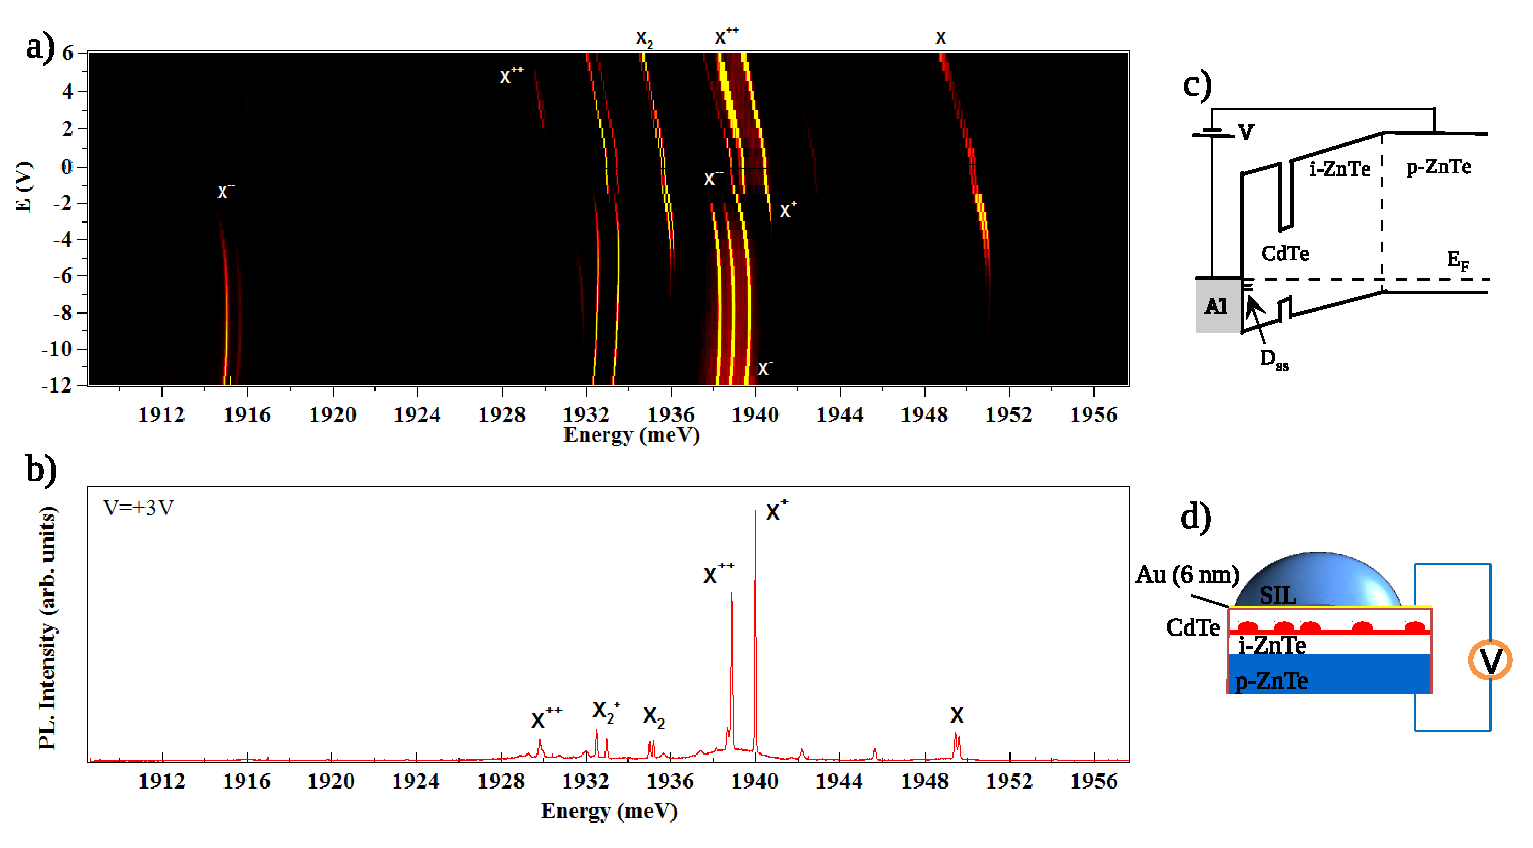
\includegraphics[width=9.5cm]{Pictures/MapEfield.eps}
	\end{center}
	\caption{(a) Evolution of the PL of a single dot under application of a bias voltage. Below are presented spectra of the dot taken under three different values of bias voltage: (a) V = $+3$ V (positively charged, top), (b) V = $+1.5$ V (neutral, middle) and (c) V = $-8$ V (negatively charged, bottom). Identification of the different species was done following ref.~\cite{BesombesIdentificXSpecies}.}
	\label{ChargeVar}
	\end{figure}

	The main result of the experiment is the appearance of different excitonic species depending on the applied electric field. We find the neutral state of the quantum dot for an applied electric field of V = -1.5 V (Fig.~\ref{ChargeVar} (c)). At this voltage, the neutral excitonic species X and X$^2$ are the strongest. Charged excitons still appear because of charge variations occuring close to the QD, injecting electron or holes inside it. Further lowering the biais voltage, the probability to of the dot to be negatively charged increase. Neutral excitonic species disappear and the peaks of the negatively charged species (X$^-$, X$^{--}$ and X$_2^-$) become dominant. A spectra taken at V = -8 V is presented on Fig.~\ref{ChargeVar} (d). One can notice that, due to the electron-electron interaction, X$^{--}$ is splitted into two group of two peaks, as was observed in InAs quantum dots~\cite{FineStructX2charge}. On the contrary, applying a positive bias voltage increases the probability to a positively charged quantum dot, maxing X$^+$ and X$^{++}$. This is shown on Fig.~\ref{ChargeVar} (b) for a bias voltage of V = +3 V. This shows that we can select efficiently the charge of a studied quantum dot applying a bias voltage on it.
%	We see for example that, for a bias voltage of +3 V (Fig.~\ref{ChargeVar} (b)), the neutral species are almost extinguish and the charged species X$^+$, X$^{++}$ and X$_2^+$ have the more intense PL. Similarly, at negative electric field, only the charged species X$^-$, X$^{--}$ and X$_2^-$ remain, X$^{--}$ and X$_2^-$ disappearing for an applied bias voltage higher than -2 V. This shows that we can select efficiently the charge of a studied quantum dot applying a bias voltage on it.
	
%		Fig.~\ref{ChargeVar} (c) gives a schematic view of the Schottky gate. In this compound, the Fermi levels of the metal, semiconductor and p-doped semiconductor align via Fermi level pinning. Applying a bias voltage to the back and front of the sample change the position of the Fermi level, and therefore the probability of injection of hole or an electron in the dot, depending on the direction of the applied voltage. Moreover, the energy barriers at the interfaces keep the current to flow in the non-doped part of the semiconductor. We can then apply an electric field on the sample, and thus control the charge of the sample, without having a current going through it.
	
	Tests were done on samples without Cr atom, and only one charge control sample containing Cr atoms was studied: dot390. It was cleaned by H$^*$ plasma. The QD layer was 5.5 ML thick and the targeted Cr concentration was 0.16\%. However, no Cr doped quantum dots were found. Some dots presenting a emission close to the one expected for Cr atoms were found, but they were revealed to not have any magnetic atom inside. The characteristic of such QDs are discussed in more details in Sec.~\ref{ChargeFluc}.
	
		\subsection{Strain-free quantum dots\label{SFD}}
		
%		The strain-free dots are formed by the interface variation of a thin (about $4ML$) CdTe quantum well (QW) between CdMgTe layers. These thickness variations will create dots, in which we will want to include a single magnetic atom. The whole structure is ideally grown on a CdTe substrate, in order to have absolutely no strain in the dots layer.
%		
%		However, there was no CdTe substrate in Tsukuba. So, we had to grow a thick layer of CdTe in top of GaAs substrate, which a lattice parameter close to CdTe, on order to have a completely relaxed surface to do our growth.
%		
%		To achieve so, we start by cleaning the GaAs substrate. It was done in four step outside the MBE chamber, all of them using an ultrasonic cleaning. It was first immersed in acetone, during 5 minutes, with the ultrasonic frequency at $43MHz$. Staying at this frequency, it was then immersed in ethanol during 5 minutes again, and then in water for the same time. We finished with a last 5 minutes cleaning in water, at $23MHz$ this time.
%		
%		Putting the substrate in a chamber, we proceeded to the last step of the cleaning: hydrogen radical (H$^*$) cleaning, created by injecting nitrogen radical in a chamber of H gas, in order to remove Ga oxyde formed at the surface while transporting the sample. We check the final composition of the gas via the electron energy using optical probing. For a H$^*$ gas, this should be round 660nm. To achieve the H radical cleaning, we heat the GaAs substrate to $400^{\circ}$C and then open the valve between the main chamber and the one containing H$^*$ gas. We exposed it for 15 minutes, and then searched for line in the RHEED pattern, to check the quality of the cleaning. during this step, and also during the growth, the sample was rotating.
%		
%		Once the cleaning process is finished, we began the growth of the thick layer of CdTe. We began by a very thin layer of ZnTe in order to relaxed some of the strain. Staying at T$_{substrate} = 400^{\circ}$C, we first opened the Zn cell for 30s, then opened both Zn and Te cells for 50s, before closing again Te cell. We then go down to T$_{substrate} = 250^{\circ}$C under Zn flux and, once the temperature was stabilized, closed the Zn cell and proceeded to the CdTe layer growth, during 1h. Finally, once this layer was grown, we protected it from oxidation by adding a thin layer of Te while the substrate temperature was going down to $5^{\circ}$C.
%		
%		For this sample, only a simple cleaning occur outside of the MBE machine. We did it in four steps, each of them lasting for 5 minutes in an ultrasonic cleaning device. We began with a cleaning acetone, at 43 kHz, followed by one in ethanol at the same frequency. We then put the substrate in water and clean it at 43 kHz. Finally, we changed the water and did the last step in water at 23 kHz, in order to clean the substrate from smaller dust particle.
%		
%		Since the surface of the GaAs is oxidized, no RHEED pattern was visible, as shown on Fig \ref{Hybrid}(a). The desoxidation was done in the MBE main chamber, in vacuum condition, using hydrogen radical (H$^*$). In order to form the radical gas, a hydrogen gas was ionized in a chamber by a RF power source of 300 W and with a frequency of 13.6 MHz. This gas composition is optically checked by probing the emission of the Balmer serie: for a pure hydrogen gas, peaks at 656 nm and 486 nm appear clearly. During the formation of this gas, the substrate temperature is raised to $400^{\circ}$C. Once the hydrogen chamber is full of H$^*$ gas, we initiate the rotation of the sample. Since the chamber was situated just under the main and linked to her, we just had to open the shutter between the two to send the radical gas onto the substrate. We exposed the substrate to this gas for 15 minutes, under a pressure of about $6\times10^{-7}$ Torr. We then checked the sample surface with RHEED, which should present a streak pattern with some dots as presented in Fig \ref{Hybrid}(b). 
%		
%		Once the cleaning of the sample was finished, we closed the H$^*$ gas chamber shutter, waited for the ultra-high vacuum to re-established in the main chamber and began the growth of the CdTe layer. We grew it in two times: one hour of growth just after the cleaning (described here) and about four hours just before the actual growth of  the quantum dots structure.

%	The barrier for strain free samples are made of CdTe. The chosen substrate for the growth was GaAs, on which we grew a layer of about 3 $\mu$m of CdTe. Growing such a thick layer guaranty that the remaining strain are in the order of $0.1\%$ \cite{StrainRelaxCdTeGaAs111,StrainRelaxCdTeGaAs100}. Moreover, a small ZnTe layer was grown between GaAs and CdTe, which accelerated the relaxation of the strains \cite{StrainRelaxZnTeGaAs001}.
	
	Since the Cr atom is really sensible to the strain state at its position, studying it in SK dots, with some remaining, was limiting the dynamic states we can study. We decided to grow strain-free dot in order to be able to study new state of the Cr spin in quantume dot. They are formed by the thickness fluctuations of a CdTe quantum well in Cd$_x$Mg$_{1-x}$Te barriers. These fluctuations form steps localizing the carriers, acting as QDs. In order to have no strain in the CdTe QW, we match the Cd$_x$Mg$_{1-x}$Te barrier on CdTe. We then chose to grow the barrier as Cd$_{0.7}$Mg$_{0.3}$Te, keeping a lattice parameter close enough to CdTe to grow thick enough barriers, and keeping enough gap difference to localize the carriers. The needed flux for this growth are shown in Tab.~\ref{FluxTempSFD}.
	
	\begin{table}[h!]
	\begin{center}		
		\begin{tabular}{| c | c |}
			\hline
			Elements & Targeted BEP (Torr) \\ \hline
			Cd & $4.5\times10^{-7}$ \\
			Mg & $1.6\times10^{-8}$ \\
			Te & $5.26\times10^{-7}$ \\
			\hline
		\end{tabular}
		\caption{Aimed flux for each cell during the growth of the strained samples.}
		\label{FluxTempSFD}
	\end{center}
	\end{table}
	
	The strain-free sample were grown on an hybrid substrate. It was made from a GaAs substrate, cleaned using H$^*$ plasma. A thin layer (about 7 nm) of ZnTe was first grown in order to help the relaxation of strains~\cite{StrainRelaxZnTeGaAs001}. We then grew a CdTe layer of about 3 $\mu$m, in order to recover the lattice parameter and not have defect close to the surface. With this thickness, the remaining strains in the layer should be of about $0.1\%$~\cite{StrainRelaxCdTeGaAs111,StrainRelaxCdTeGaAs100}. The RHEED taken after the growth of the CdTe layer (Fig.~\ref{Hybrid} (d)) shows sharp straight line, suggesting the recovery of a flat surface. Since we did a large quantity of hybrid substrate, to be cut later to do multiple samples with it, a protective layer of amorphous Te was grown on the surface to keep it from being damaged outside the MBE chamber.

	\begin{figure}[h!]
	\begin{center}
		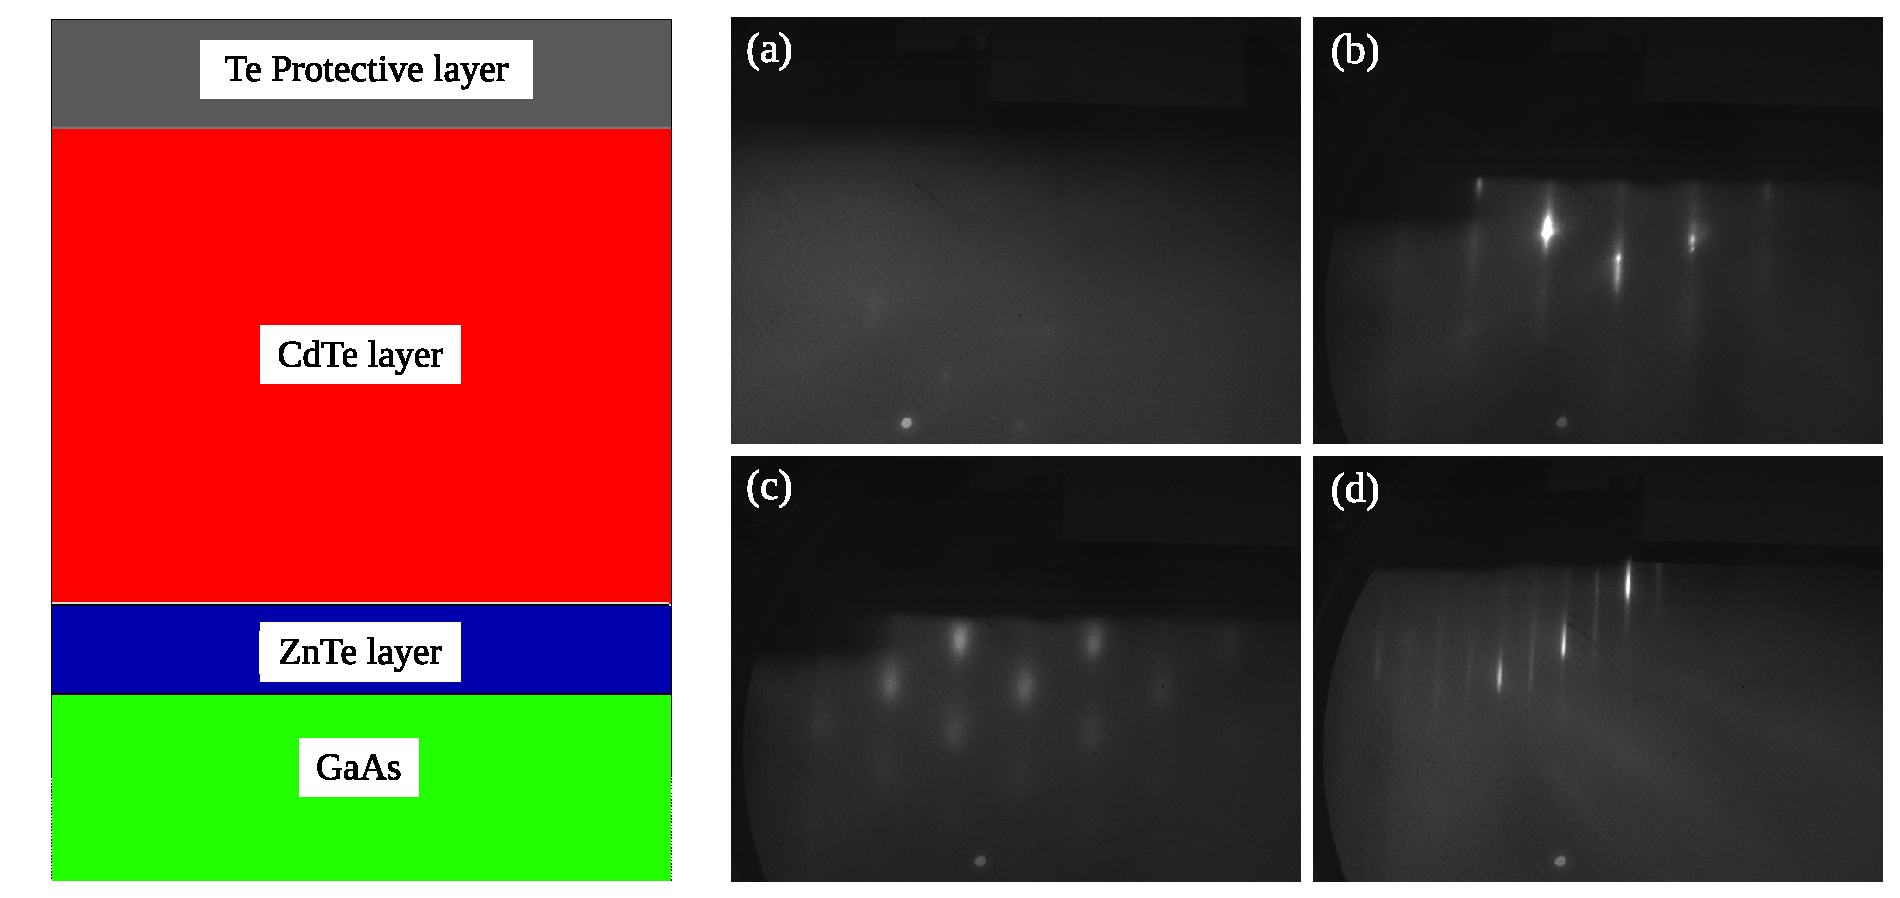
\includegraphics[width=14cm]{Pictures/HybridSubstrate.eps}
	\end{center}
	\caption{Left: Layer structure of the hybrid substrate with its protective Te cap.
		Right: RHEED pattern taken at different key moment of the growth: (a) before H$^*$ cleaning of GaAs, (b) after H$^*$ cleaning of GaAs, (c) after the growth of the ZnTe layer, (d) after the growth of the CdTe layer.}
	\label{Hybrid}
	\end{figure}
		
%		This first part of the growth took place on a rotating sample. It only take about 15 ML of ZnTe on GaAs for the II-VI compound go back to its original lattice parameter \cite{StrainRelaxZnTeGaAs001}. Moreover, CdTe over ZnTe has a critical thickness of 5 ML \cite{CritThickCdTeZnTe}. So, to accelerate the relaxation of strain, we decided to grow a thing layer of ZnTe above the GaAs, before growing the CdTe thick layer. We lowered the substrate temperature to $320^{\circ}$C and opened the Zn cells for 30s with a BEP of $7.05\times10^{-7}$ Torr in order to flatten the surface. We then opened the Te cells, with a BEP of $5.21\times10^{-7}$ Torr, along with the Zn cell during 50s to grow the ZnTe layer in excess of Zn, making a layer about 7.2 nm thick.
%		
%		We then went to the growth of the first CdTe layer. We lowered again the substrate temperature to $250^{\circ}$C, under Zn flux. Once stabilized at the temperature, we closed Zn cells and open the Cd and Te cells for 1h. The Te cell had the same flux as previously, while the Cd cells had a flux of $4.72\times10^{-7}$ Torr. This layer was 633 nm thick, grown at 0.54 ML.s$^{-1}$. In order to protect the surface, we deposit an amorphous protective layer of Te above it, while decreasing the substrate temperature.
		
%	As said in the introduction, the strain free dots are formed by thickness variation of a CdTe QW surrounded by CdMgTe barrier. In order to have to good confinement while keeping a close enough lattice constant, we chose to use Cd$_{0.7}$Mg$_{0.3}$Te. Therefore, the first step of the growth was to chose the flux for the growth. We went through a process of trial and error, growing several samples and testing their composition with Electron Probe Mico-Analysis and X-Ray diffraction, as well as the thickness grown with a step gauge, in order to estimate the growth speed. Since we wanted to grow Cd$_{0.7}$Mg$_{0.3}$Te, we began the test with a ration Te:Cd of 1:0.7 and a ratio Te:Mg of 1:0.3. After five round of adjustment, we achieve the growth of Cd$_{0.7}$Mg$_{0.3}$Te, settling with the targeted flux presented in Tab.\ref{FluxTempSFD}.
%	For the settled Mg flux, the step gauge indicated a grown thickness of $520 \pm 5$ nm. Since we grew the test layer during 1h, we found a growing speed of about 0.15 nm.s$^{-1}$.
	
	For the actual growth of strain free samples, we began to heat the substrate temperature to 300$^{\circ}$C, in order to remove the protective amorphous Te layer. We waited a few seconds at this temperature to remove all the deposited Te, and then resumed the heating to go to $360^{\circ}$C. Starting at $320^{\circ}$C, we opened the Te cells in order to stabilize the surface. When the substrate temperature was stabilized at $360^{\circ}$C, we opened the Cd cells and grew a 2.35 $\mu$m layer of CdTe on top of the 3 $\mu$m grown on the hybrid substrate, in order to be as close as possible of a total lattice parameter recovery ~\cite{StrainRelaxCdTeGaAs111,StrainRelaxCdTeGaAs100}.
	
	\begin{figure}[h!]
	\begin{center}
		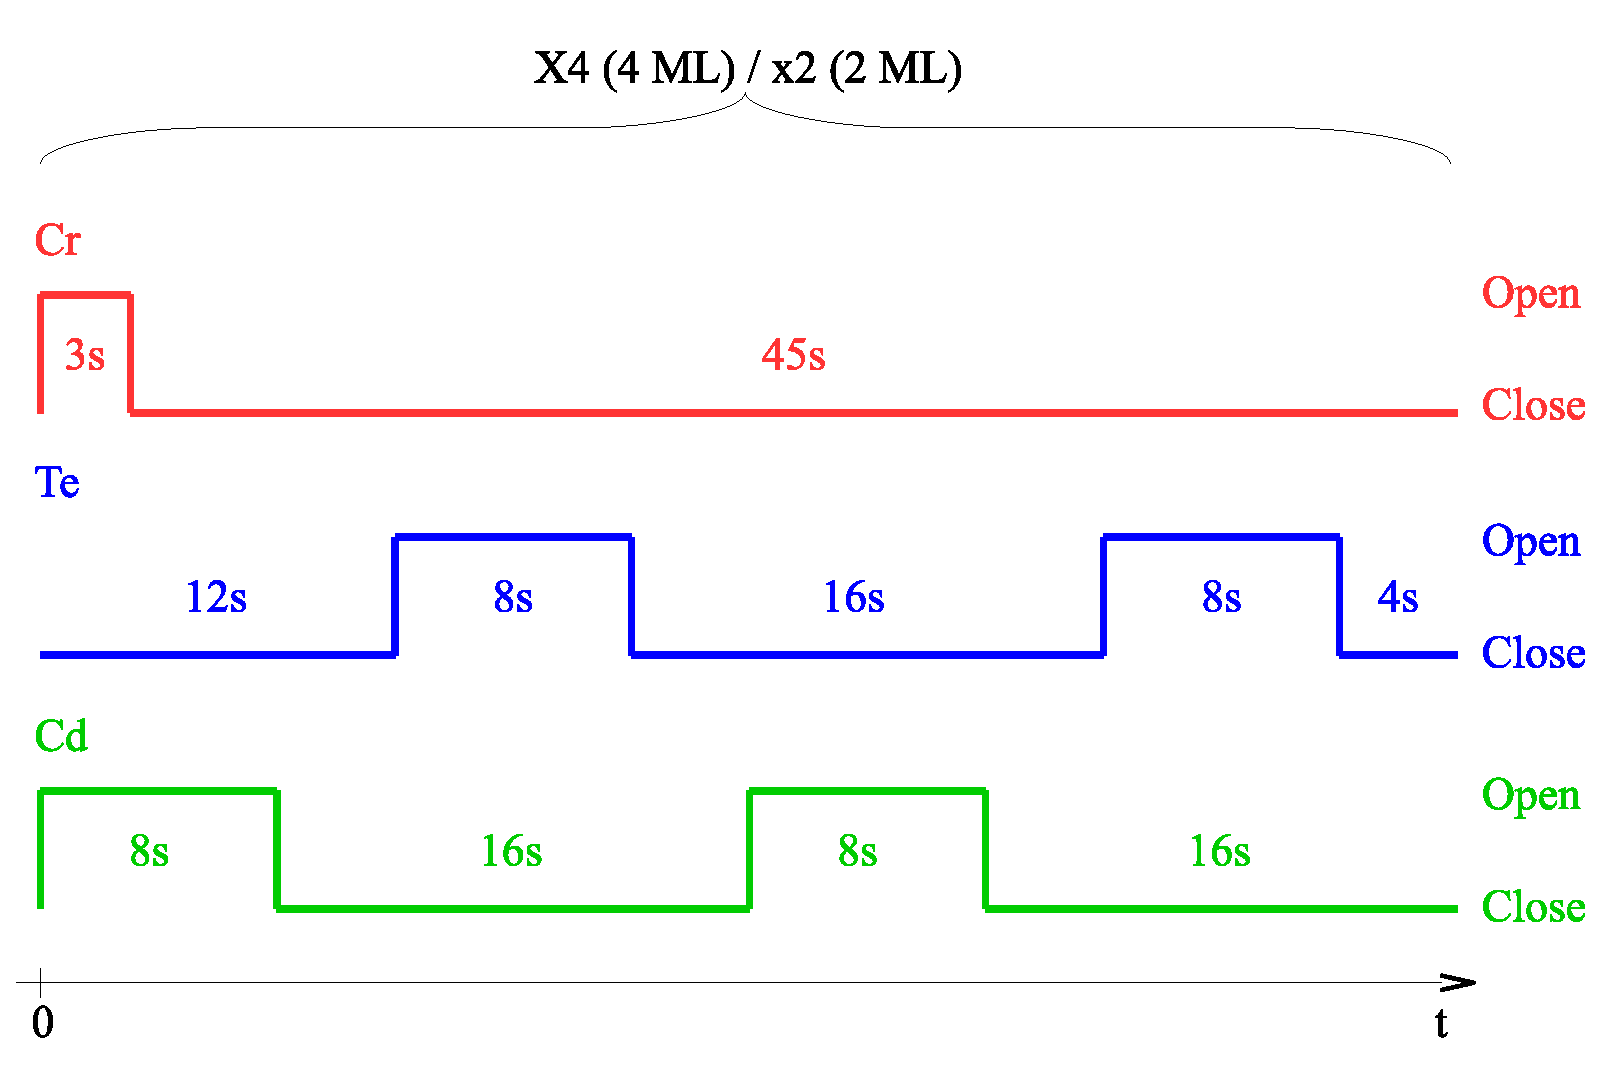
\includegraphics[width=10cm]{Pictures/RecipeSFD.eps}
	\end{center}
	\caption{Opening and closing cycles of each cell for the ALE of strain free (Cd,Cr)Te samples.}
	\label{RecipeSFD}
	\end{figure}
	
	We grew the first Cd$_{0.7}$Mg$_{0.3}$Te barrier on this buffer layer. The critical thickness of Cd$_{0.7}$Mg$_{0.3}$Te on CdTe is not exactly known. However, Cd$_{0.96}$Zn$_{0.04}$Te has a lattice parameter close to Cd$_{0.7}$Mg$_{0.3}$Te, and we expect their critical thickness to be close. In order to be safe, we chose to limit ourselves to a maximum cumulated thickness of 130 nm~\cite{CritThickCdTeCdZnTe}. We chose to grow 40 nm below the QW, and 90 nm above it, in order to have a thicker protective layer.
%Moreover, it was shown on Mn that a thick layer above was better for the hole trapping.

	Once the 40 nm barrier layer was grown, we lowered the substrate temperature under Te flux. Growing the QW layer in a Te environment smooth the surface layer of the sample and help having a flat surface to grow the well. Once the substrate temperature reach respectively $295^{\circ}$C, we began the ALE of the QW. Two QW thickness was tested: either 4 ML or 2 ML. In both case, the growth was done growing CdTe layer as done for the strained samples, opening the Cr cell for 3 s for one cycle every two cycles. The whole recipe is described in Fig.~\ref{RecipeSFD}.
	
	We then raised the substrate temperature up to $360^{\circ}$C, under a Te flux, in order to proceed to the growth of the upper barrier, acting also as a protective layer. The opening time was there calculated to grow 90 nm of Cd$_{0.7}$Mg$_{0.3}$Te.

	\subsubsection*{Optical characterization}
	
	Four sample of strain-free dots doped with Cr were produced, listed in Tab.~\ref{SFDsamples}.
	
	\begin{table}[h!]
		\begin{center}
			\caption{List of sample grown trying to incorporate Cr in SFD dots.\label{SFDsamples}}
			\begin{tabular}{M{2cm}|M{2.5cm}|M{3.5cm}|M{3cm}}
				Sample & \# CdTe MLs & Cr aimed concentration (\%) & Probability of Cr-doped QD \\
				\hline
				SFD4 & 4 & 0.35 & None found \\
				SFD5 & 2 & 0.15 & None found \\
				SFD6 & 2 & 0.54 & None found \\
				SFD7 & 2 & 0.35 & None found \\
				SFD8 & 2 & 0.75 & None found
			\end{tabular}
		\end{center}
	\end{table}
	
%	\begin{figure}[h!]
%	\begin{center}
%		\includegraphics[width=10cm]{../FillingPicture.png}
%	\end{center}
%	\caption{Example of dot fin in SFD}
%	\label{ChargeVar}
%	\end{figure}
	
	The sample presented thin and intense peaks, as shown in Fig.~\ref{SpectraSFD}. It hints at a better confinement of the carriers in the QDs than what have been expected from dots formed by the thickness variation of a quantum well. This may be caused by higher steps than expected at the CdTe/Cd$_{0.7}$Mg$_{0.3}$Te interface.
	
	\begin{figure}[h!]
	\begin{center}
		\includegraphics[width=10cm]{Pictures/SFDSpectra.eps}
	\end{center}
	\caption{(a) Macro-photoluminescence of a sample containing strain free dots. (b) Examples of spectra taken in such a sample.}
	\label{SpectraSFD}
	\end{figure}
	
	As discussed in Sec.~\ref{XMn}, the presence of a magnetic atom splits the emission of the exciton into several peaks, the number depending on the spin of the magnetic atom. However, such complex was not found in the strain-free samples. The cause of this absence could lie in the absence of strain. In SK dots, the presence of strains increases the probability of the Jahn-Teller deformation to occur along the $z$ axis. In strain-free dots, all direction are equivalent, and we expect two third of the Cr-doped dots to be undetectable because they are quantized in the plane, creating no splitting visible in our setup.
	
	In order to counter that, it was proposed to slightly strain the quantum well. This might be done by growing the sample on Cd$_{0.96}$Zn$_{0.04}$Te instead of CdTe. The lattice parameter of Cdte and Cd$_{0.96}$Zn$_{0.04}$Te are close, so the strain it will create in the lattice should remain weak. They should however be enough to increase the probability of a deformation along the $z$ axis, making more dots visible in our setup.
	
	\section*{Conclusion}
	
	We saw in this chapter how we grew the samples studied in the next chapters. The samples were characterized in Grenoble and the Cr concentration in the samples was refined through a feedback loop between Grenoble and Tsukuba. More test have to be done with a targeted concentration around 0.10\%.
	
	Two other kind of sample were also grown: charge control samples and strain-free dots. Both of them encountered mild success. We were able to apply an electric field on charge control samples, but not dots containing a single Cr atom were found. In the strain-free dots, we saw the dot had a good localisation of carriers, but no Cr-doped dots were found either. More test have to be done in both of them to be able to use them for an optical study of single Cr atoms in CdTe quantum dots.
%
% 	We used the characterization of the samples done in Tsukuba to narrow down on a Cr flux for the growth of Cr-doped QDs, and we decided to aim for a Cr estimated concentration in the sample of  0.17\%. We then went to two other kind of sample: one enabling the application of an electric field on the dots, and one with strain free dots. The charge control samples growth was a partial success: we were able to apply an electric field on the sample, but no dot containing a single Cr was found. Strain-free dot presented promising fine peaks in their emission, but we were not able to find Cr in them either. More experiments will be done in order to successfully grow sample with the possibility of charge control, and strain-free dots.
	
	In the next chapters, we will study the optical properties and the spin dynamics in the magnetic QDs grown in Grenoble (Chap.~\ref{CoDynMn}) and Tsukuba (Chap.~\ref{MagOptStud} and \ref{CrDyn}).

\printbibliography

\end{document}